\section{Simulations}
\label{sec:simulations}

%We evaluate our approximation algorithms -- described in Section \ref{sec:approx} -- using simulations. 
We evaluate our approximation algorithms using simulations. 
For each algorithm, we determine the number of nodes that are observed by placing $k$ PMUs on IEEE bus systems $14$, $30$, $57$, $118$ and $300$,
{\footnote {\small http://www.ee.washington.edu/research/pstca/}} as well as synthetic graphs generated by using these IEEE graphs as templates.

A synthetic graph is generated from a given IEEE graph in the following manner: for each bus system, we start with the original graph and then randomly choose pairs of edges and ``swap''
their endpoints. Specifically, given two disjoint edges $(u,v),(w,y)$, an {\em edge swap} converts these to $(u,y),(v,w)$. We swap edges until the original graph and generated graph share no edges. Note that this edge-swapping procedure ensures that the degree distribution of each generated graph is exactly the same as the degree distribution
of the original bus system. 


When possible we compare the results of our greedy algorithms to an optimal placement of PMUs. The optimal placement was computed in brute-force manner, by enumerating all valid placements of $k$ PMUs and
then selecting the PMU placement that observes the maximum number of nodes.
For \xval and \xvalparts, we ignore PMU placements that do not meet cross-validation requirements.
%For \xval and \xvalparts, we ignore PMU placements which do not meet the cross-validation rules described in Section \ref{subsec:xval}. 
Because this brute-force algorithm has exponential running time in the size of the input, we were unable to determine optimal PMU placements for larger $k$ values in synthetic graphs generated
from the IEEE $118$ bus system and the actual IEEE $118$ bus system. For this reason, the ``optimal'' curve stops abruptly in Figure \ref{fig:bus118}, Figure \ref{fig:xvbus118}, and Figure \ref{fig:all118}. 

%We continue this procedure until $\pm 0.10(\overline{x})$ -- where $\overline{x}$ is the mean number of observed nodes using $k$ PMUs -- falls within the $90\%$ confidence interval.

We first present the results for the synthetic graphs and then briefly discuss the results for the actual IEEE bus systems. 
For the synthetic graphs, each data point is generated as follows. For a given number of PMUs, $k$, we generate a graph, place $k$ PMUs on the graph, and then determine the number of observed nodes. 
We continue this procedure until $[0.9(\overline{x}),1.1(\overline{x})]$ -- where $\overline{x}$ is the mean number of observed nodes using $k$ PMUs -- falls within the $90\%$ confidence interval.

The results for \maxinc are shown in Figure \ref{fig:maxinc-res}. Figure \ref{fig:xv-res} shows the results for \xval and \xvalparts. The $90\%$ confidence interval is shown in each plot.
The simulation results for graphs based on IEEE bus $14$ are omitted because each greedy algorithm always correctly finds the optimal solution. Also, we do 
not show the IEEE bus $300$ results because the graph size prevented us from running the brute-force optimization algorithm. 

Our greedy algorithms perform well. For the \maxinc problem, on average, the greedy algorithm is within $96.5\%$ of optimal.  Greedy 
is never below $86\%$ of the optimal solution, and in most cases gives the optimal result.
Likewise, for \xvalpart the greedy solution always gives a solution at least $84 \%$ of optimal.  On average the \xvalpart greedy algorithm is within $97\%$ of optimal
and in about half the cases, the greedy solution is optimal. 
These results suggest that the simple greedy approach works well in practice. Typically, greedy algorithms fail because they commit to a choice too early
and do not reconsider earlier decisions.  Our results suggest that this is not the case for \maxincs, \xvals, and \xvalparts.

Surprisingly, we found that {\tt optimal} for \xvalpart observed close to the same number of nodes as {\tt optimal} for \maxincs. Across
the same $k$ values, on average {\tt optimal} for \xvalpart observed only $12\%$ fewer nodes than {\tt optimal} for \maxincs. This suggests that the restriction that all nodes
are cross-validated does not have a significant effect on the resulting number of observed nodes.


%Xu and Abur \cite{Xu05} use simulations to evaluate their integer linear programming approach for PMU placement, for the PDS problem.  Note the PDS problem corresponds to \maxinc when $k$ is sufficient to cover 
%all nodes. Their algorithm results in $4$, $10$, $17$, and $32$ PMUs on IEEE bus $14$, $30$, $57$, and $118$, respectively.  In terms of number of PMUs for full system observability, this marks an increase of $200\%$, $333\%$, $334\%$, $332\%$, respectively, 
%when compared to our greedy solution for the corresponding buses. 

\begin{figure*}[t]
  \begin{center}
    \subfigure[Graphs based on IEEE Bus $30$]{\label{fig:bus30}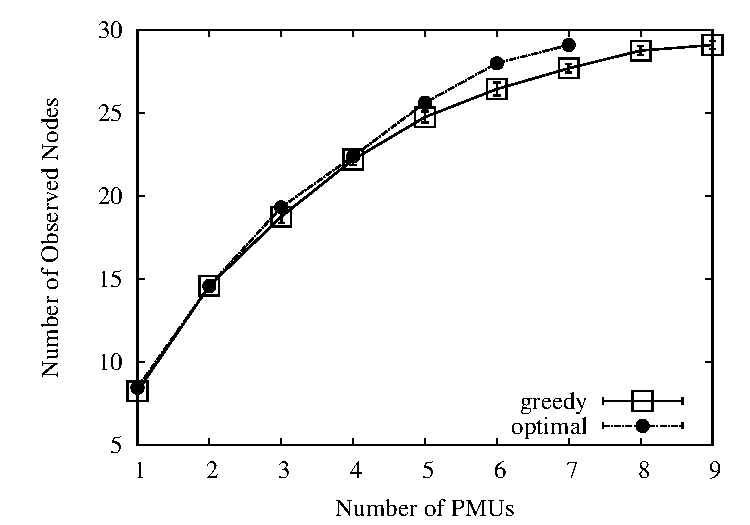
\includegraphics[scale=0.49]{figs/bus30.pdf}}
    \subfigure[Graphs based on IEEE Bus $57$]{\label{fig:bus57}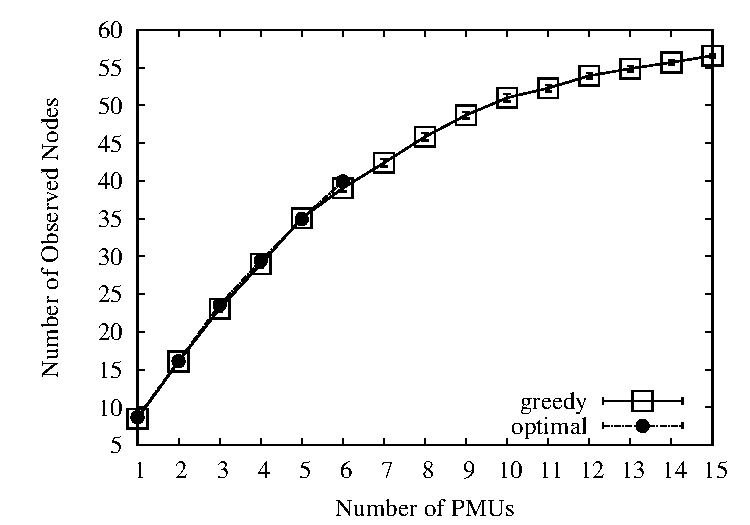
\includegraphics[scale=0.49]{figs/bus57.pdf}}
    \subfigure[Graphs based on IEEE Bus $118$]{\label{fig:bus118}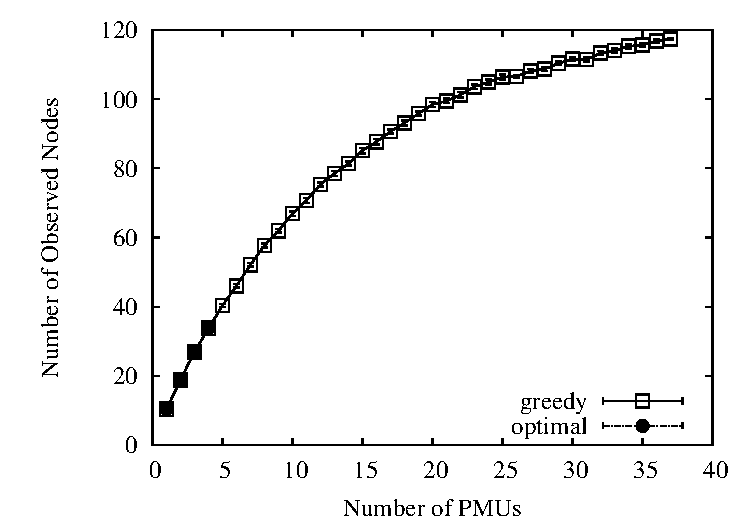
\includegraphics[scale=0.49]{figs/bus118.pdf}}
  \end{center}
	\caption{Simulation Results for \maxincs.  The $90\%$ confidence interval is shown.}
  \label{fig:maxinc-res}
\end{figure*}

\begin{figure*}[t]
  \begin{center}
    \subfigure[Graphs based on IEEE Bus $30$]{\label{fig:xvbus30}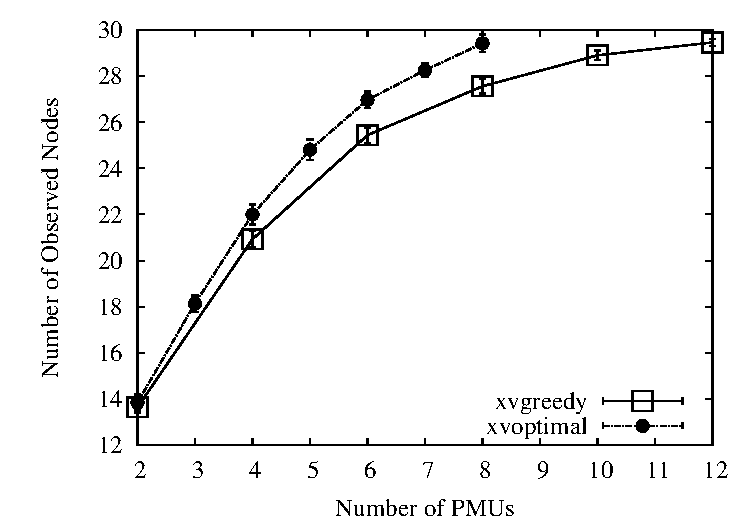
\includegraphics[scale=0.49]{figs/xvbus30.pdf}}
    \subfigure[Graphs based on IEEE Bus $57$]{\label{fig:xvbus57}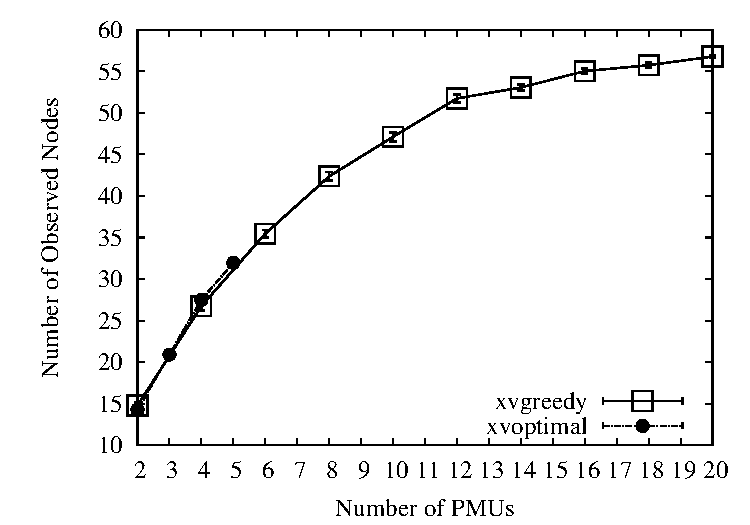
\includegraphics[scale=0.49]{figs/xvbus57.pdf}}
    \subfigure[Graphs based on IEEE Bus $118$]{\label{fig:xvbus118}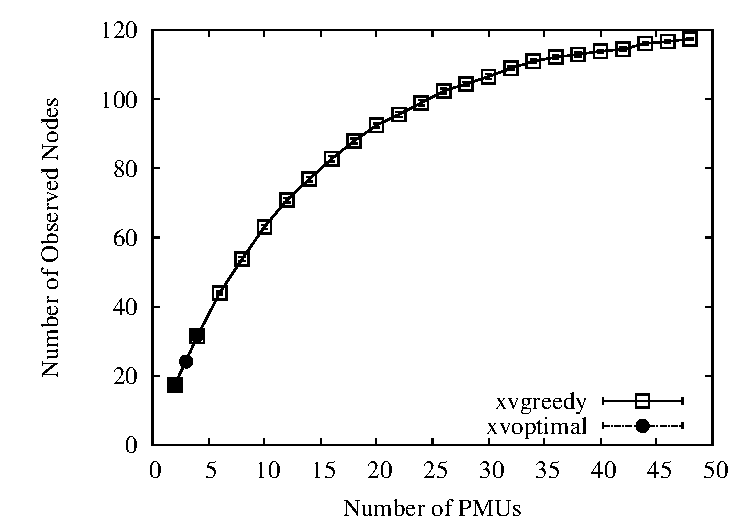
\includegraphics[scale=0.49]{figs/xvbus118.pdf}}
  \end{center}
	\caption{Simulation Results for \xval and \xvalparts. {\tt xvgreedy} refers to the greedy algorithm with cross-validation and {\tt xvoptimal} is for the brute-force optimal
	algorithm with cross-validation. The $90\%$ confidence interval is shown. }
  \label{fig:xv-res}
\end{figure*}

We also ran simulations over the actual IEEE bus systems. We found the trends between our greedy and {\tt optimal} algorithms were consistent with the results from our simulations over synthetic graphs. 
For example, Figure \ref{fig:all118} shows the number of observed nodes for greedy
and {\tt optimal} for both the \maxinc and \xvalpart problems over IEEE bus $118$.  In both cases, the greedy algorithm observes nearly as many nodes as the {\tt optimal} solution. 
In many cases, greedy yields the optimal placement. These results are consistent with our findings for IEEE bus system $14$, $30$, and $57$. 



\begin{figure}[t]
\centering
\includegraphics[scale=0.49]{figs/all118.pdf}
%\includegraphics[scale=0.65]{figs/all118.pdf}
\caption{Simulation results for \maxinc and \xvalpart using IEEE bus $118$.}
\label{fig:all118}
\end{figure}




%\begin{figure*}[t]
%  \begin{center}
%    \subfigure[IEEE Bus $30$]{\label{fig:bus30}\includegraphics[scale=0.47]{figs/allbus30.pdf}}
%    \subfigure[IEEE Bus $57$]{\label{fig:bus57}\includegraphics[scale=0.47]{figs/allbus57.pdf}}
%    \subfigure[IEEE Bus $118$]{\label{fig:bus118}\includegraphics[scale=0.47]{figs/allbus118.pdf}}
%  \end{center}
%	\caption{Simultation Results for IEEE Bus $30$, $57$, and $118$.} 
%  \label{fig:all-res}
%\end{figure*}

